\documentclass[10pt,handout,english]{beamer}
\usepackage[compatibility=false]{caption}
\usepackage[english]{babel}
\usepackage[backend=biber,style=numeric-comp,sorting=none]{biblatex}
\usepackage{amsmath}
\usepackage{blkarray}
\newcommand{\matindex}[1]{\mbox{\scriptsize#1}}
\usepackage{amssymb}
\usepackage{graphicx,caption,copyrightbox}
\usepackage{hyperref}
\usepackage{color}
\usepackage{subcaption}
\usetheme{Berlin}
\beamertemplatenavigationsymbolsempty
\captionsetup{justification=centering, labelfont=sc, labelsep=endash}

\title[Default Classification]{Classifying Default Application for \\Peer-to-Peer Bitcoin Loans\\}
\subtitle{Competitive Machine Learning}
\author[Baptiste O'Jeanson]{Baptiste~O'Jeanson}
\institute[Potsdam University]{Institute of Computer Science}
\date{}
\subject{Computer Science}

\AtBeginSubsection[]
{
  \begin{frame}
    \frametitle{Table of Contents}
    \tableofcontents[currentsection, currentsubsection, subsubsectionstyle=hide]
  \end{frame}
}

\expandafter\def\expandafter\insertshorttitle\expandafter{%
  \insertshorttitle\hfill%
  \insertframenumber\,/\,\inserttotalframenumber}

\begin{document}

	\maketitle

	\begin{frame}
	\frametitle{Table of Contents}
	\tableofcontents[currentsection, sectionstyle=show, subsectionstyle=show, subsubsectionstyle=hide]
	\end{frame}

	\section{Introduction}
		\begin{frame}
		\frametitle{Introduction}
			With the arrival of the digital currency Bitcoin, peer-to-peer lending platform were born.\\~\\
			Their main problems are :
			\begin{itemize}
				\item Identifying fraudulent online loan applications
				\item Predicting the default risk of online loan applications\\~\\
			\end{itemize}
			For the project, we used the data of the lending platform Bitbond.
		\end{frame}


	\section{Problem Setting}
		\begin{frame}
		\frametitle{Problem Setting 1/2}
			Predict the risk, at the application time of the loan, that a person will default the terms of this precise loan according to :\\
			\begin{itemize}
				\item his personal data (location, gender, employment, etc.) and/or
				\item his past experience of loan (if he has) and
				\item the similar past loans that other people asked for.\\~\\
			\end{itemize}
			$X = \bordermatrix{~ & \underset{\downarrow}{feature_1} & & \underset{\downarrow}{feature_p} \cr
			loan_1 \rightarrow & x_{1,1} & \dots & x_{1,p} \cr
			~ & \vdots & \ddots & \vdots \cr
			loan_n \rightarrow & x_{n,1} & \dots & x_{n,p} \cr}$
		\end{frame}

		\begin{frame}
		\frametitle{Problem Setting 2/2}
			\begin{itemize}
				\item Matrix of loans X  of shape (n,p) : n loans described by p features
				\item Vector of labels Y of shape (n,1) and $Y = \{0, 1\}$
				\item Model $f_\theta:X\rightarrow\{0,1\}$\\~\\
				\item Find model parameters that minimize regularized empirical risk :\\
				$\theta^*=argmin_\theta\sum_{i=1}^n l(y_i,f_\theta(x_i)) + \lambda\Omega(\theta)$\\~\\
				\item Loss function $l(f_\theta(x_i),y_i)$ and regularization are :
				\begin{itemize}
					\item Logistic loss + $l_2$ regularization: logistic regression
					\item Hinge loss + $l_2$ regularization: SVM
				\end{itemize}
			\end{itemize}

		\end{frame}

		\subsection{Evaluation}
		\begin{frame}
		\frametitle{Evaluation 1/2}
			\begin{block}{Cross validation :}
				5-fold cross validation on the borrowers (one same borrower is either in the training set or the testing set but not both) :
				\begin{itemize}
					\item Build a classifier on a training set
					\item Predict the probabilities or decision function of each label on a testing set
					\item Compute the logistic loss (if the classifier is a logistic regression)
					\item Compute hinge loss (if SVM)
					\item Compute the area under the Receiver Operating Characteristic curve (ROC-AUC score)
				\end{itemize}
			\end{block}
		\end{frame}

		\begin{frame}
		\frametitle{Evaluation 2/2}
			\begin{columns}[c]
				\column{.4\textwidth}
					\begin{figure}[h!]
			        	\centering
			        	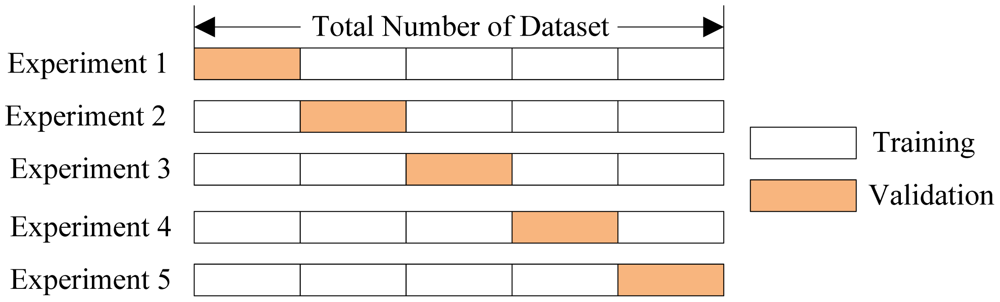
\includegraphics[width=1.25\textwidth]{5_fold_cv.png}
			            \label{fig:netflix}
			            \caption{5-fold cross validation.}
			        \end{figure}
				\column{.6\textwidth}
					\begin{figure}[h!]
			        	\centering
		            	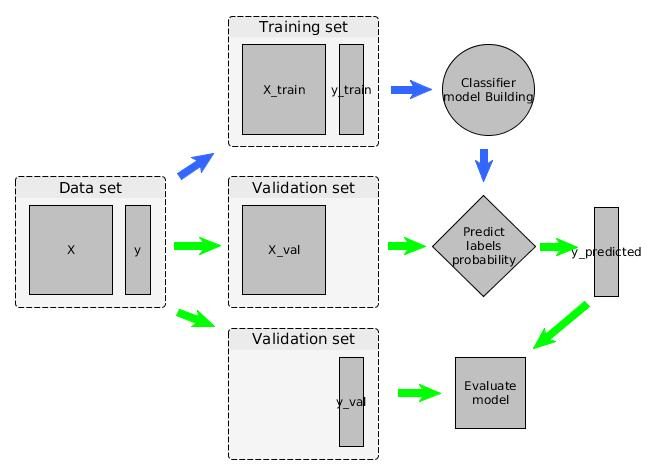
\includegraphics[width=0.85\textwidth]{cv_process.jpg}
		                \label{fig:netflix}
		                \caption{Cross validation process for one fold.}
		            \end{figure}
			\end{columns}
		\end{frame}

		\subsection{Data}
		\begin{frame}
		\frametitle{Data 1/2}
			Data set containing 2177 loans. Each loan consists of :
			\begin{columns}[c]
				\column{.5\textwidth}
					\begin{itemize}
						\item status
						\item term in months
						\item purpose from a given set
						\item project description
						\item loan amount
						\item currency (Bitcoin or USD)
						\item number of rates to pay and already paid
						\item borrower ID
					\end{itemize}
				\column{.5\textwidth}
					\begin{itemize}
						\item publishing and funding time of the loan
						\item borrower's employment
						\item borrower's net income in local currency
						\item borrower's address
						\item social media connection between the borrower and the Bitbond page
					\end{itemize}
			\end{columns}
		\end{frame}

		\begin{frame}
		\frametitle{Data 2/2}
			Among those 2177 loans :
			\begin{itemize}
				\item 608 have either defaulted (49), fully paid back (391), charged off (119) or 90 days late (49) status
				\item We consider those 608 loans for the classification task (with fully paid back label (65\%) against the rest (35\%))
				\item 521 distinct borrowers whose 446 have an address defined by their latitude and longitude
			\end{itemize}
		\end{frame}


	\section{Features and Classification models}
		\subsection{Feature Engineering}
		\begin{frame}
		\frametitle{Feature Engineering 1/4}
			The features used are the following :
			\begin{itemize}
				\item Categorical features :
				\begin{itemize}
					\item the term of the loan
					\item social media connection between the borrower and the Bitbond page (linkedin, facebook, twitter, paypal, ebay)
				\end{itemize}
				\item Textual feature : the project description
				\item Time feature : the published date
			\end{itemize}
			$\Rightarrow$ represented a 608 by (15 + 20) matrix
		\end{frame}

		\begin{frame}
		\frametitle{Feature Engineering 2/4}
			Why not use the ``income'' feature or the ``address'' ?
			\begin{itemize}
				\item Use numbeo to get for each country (presented in the dataset) their ``Average Monthly Disposable Salary''
				\item But a lot of work about checking the data provided by numbeo and bitbond concerning the currency
				\item After checking the more I could, no difference made by feature ``ratio income over average salary'' in the classification
			\end{itemize}
			Why not the other features ? No improvements in the classification.
		\end{frame}

		\begin{frame}
		\frametitle{Feature Engineering 3/4}
			\begin{itemize}
				\item Textual feature `project description' processing :
					\begin{enumerate}
						\item Tokenization
						\item Compute Part-of-Speech Tagging
						\item Use POS Tagging to improve Lemmatization
						\item Remove stopwords and puntuation
						\item Transform the normalized `description' in the bag-of-words representation
						\item Apply Latent Dirichlet Allocation on the bag-of-words with 20 topics
					\end{enumerate}
				\item Time feature `published date' :
					\begin{enumerate}
						\item Extract the first date in time of the published date
						\item Subtract it to all other published date
						\item Transform the resulting date into the number month
					\end{enumerate}
			\end{itemize}
		\end{frame}

		\begin{frame}
		\frametitle{Feature Engineering 3/4}
			Is the risk of default correlated to the location of the borrower ? $\rightarrow$ No!
			\begin{figure}[h!]
            	\centering
                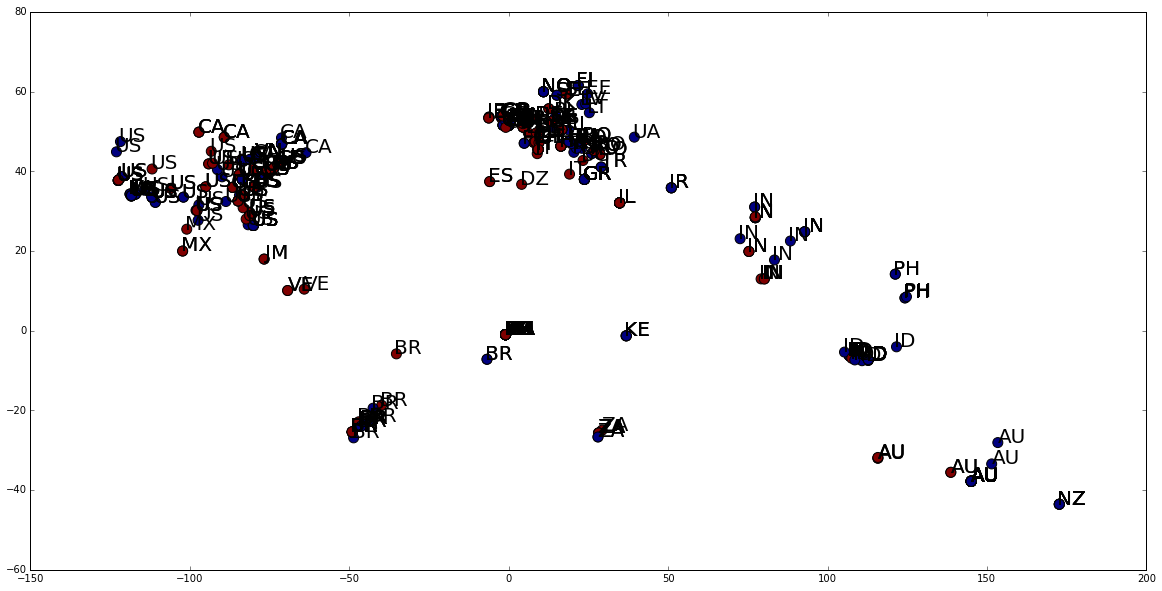
\includegraphics[width=\textwidth]{location.png}
                \caption{Map of the borrower location with label being default or not}
			\end{figure}
		\end{frame}

		\subsection{Classification models}
		\begin{frame}
		\frametitle{Classification models}
			Supervised model :
			\begin{itemize}
				\item To reduce the matrix dimension : Linear Discriminant Analysis
				\item To predict the risk of default of a new loan :
				\begin{itemize}
					\item Logistic regression
					\item Linear Support Vector Classification (SVM based on liblinear implementation)
					\item C-Support Vector Classification (SVM based on libsvm implementation)
				\end{itemize}
			\end{itemize}
		\end{frame}

		\begin{frame}
		\frametitle{Dimensionality reduction : Linear Discriminant Analysis with 2 components}
			\begin{figure}[h!]
            	\centering
                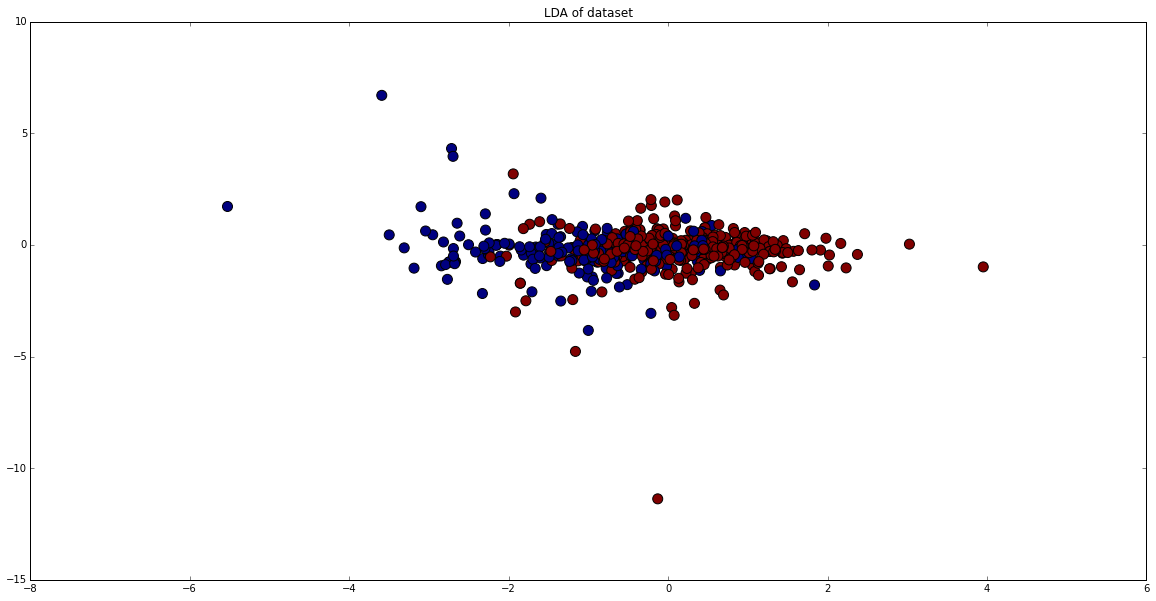
\includegraphics[width=\textwidth]{lda.png}
                \caption{Linear Discriminant Analysis with 2 components}
			\end{figure}
		\end{frame}

		\begin{frame}
		\frametitle{Dimensionality reduction : Principal Component Analysis with 2 components}
			\begin{figure}[h!]
            	\centering
                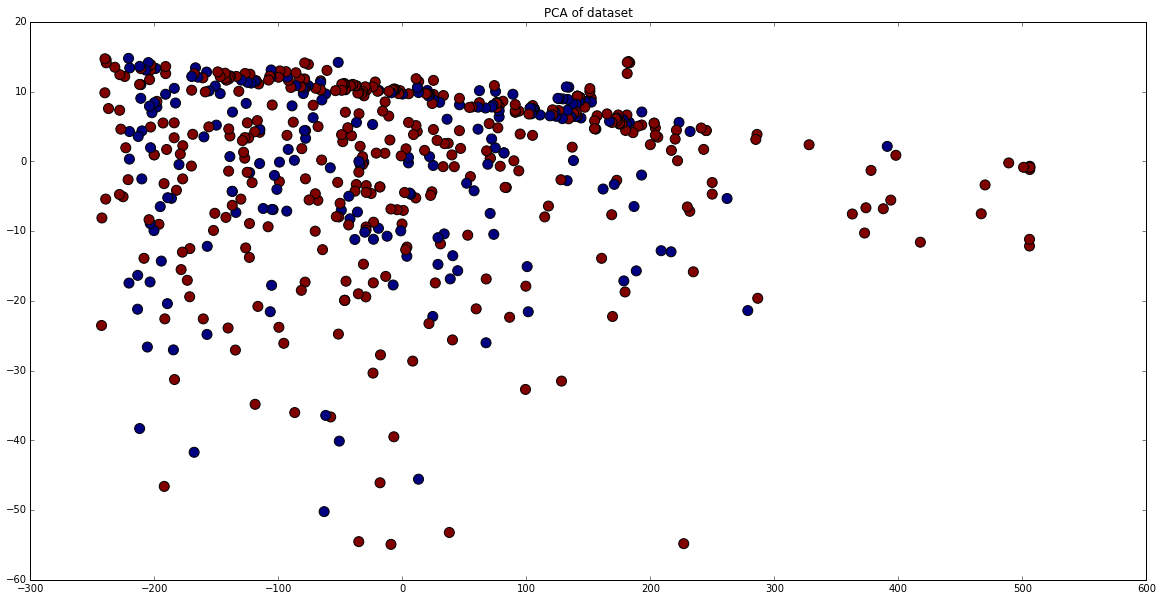
\includegraphics[width=\textwidth]{pca.png}
                \caption{Principal Component Analysis with 2 components}
			\end{figure}
		\end{frame}

		\begin{frame}
		\frametitle{Dimensionality reduction : Kernel Principal Component Analysis with 2 components}
			\begin{figure}[h!]
            	\centering
                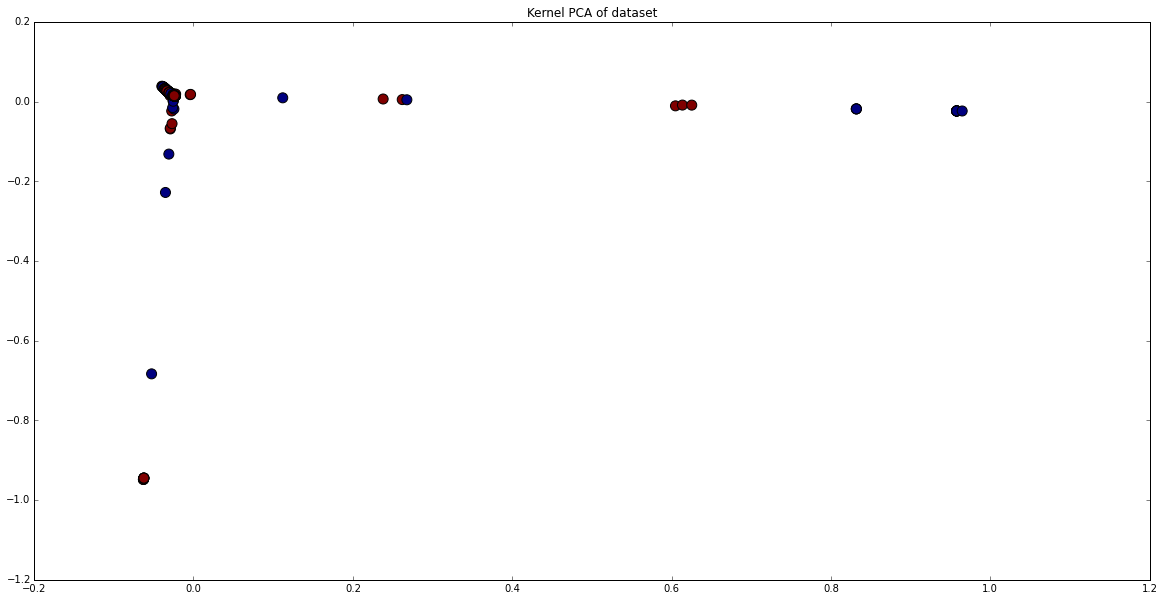
\includegraphics[width=\textwidth]{kernel_pca.png}
                \caption{Kernel Principal Component Analysis with 2 components and \href{http://scikit-learn.org/stable/modules/metrics.html\#metrics}{RBF kernel}}
			\end{figure}
		\end{frame}

		\begin{frame}
		\frametitle{Dimensionality reduction : Singular Value Decomposition with 2 components}
			\begin{figure}[h!]
            	\centering
                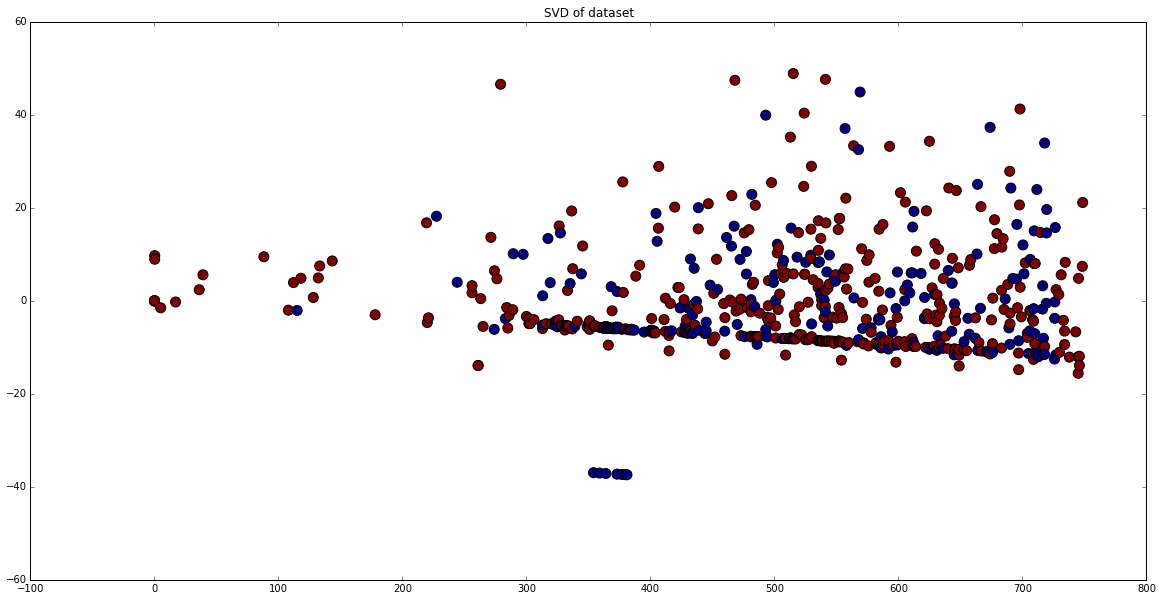
\includegraphics[width=\textwidth]{svd.png}
                \caption{Singular Value Decomposition with 2 components}
			\end{figure}
		\end{frame}

	\section{Evaluation}
		\subsection{Loss function}
		\begin{frame}
		\frametitle{Loss function}
			\begin{itemize}
				\item Log loss score :
				\begin{itemize}
					\item Logistic regression : 0.56 (mean on the 5-fold)
					\item SVC : 0.56 (mean on the 5-fold)
				\end{itemize}
				\item Hinge loss score :
				\begin{itemize}
					\item SVC : 0.65 (mean on the 5-fold)
					\item LinearSVC : 0.70 (mean on the 5-fold)
				\end{itemize}
			\end{itemize}
			Remark : The Logistic regression model of sklearn is based on the same library (liblinear) as SVC model, that is why we can compute for both the probabilities of each labels. (Not possible with LinearSVC based on libsvm)
		\end{frame}

		\subsection{Logistic Regression evaluation}
		\begin{frame}
		\frametitle{Logistic Regression evaluation}
		\begin{figure}[h!]
        	\centering
            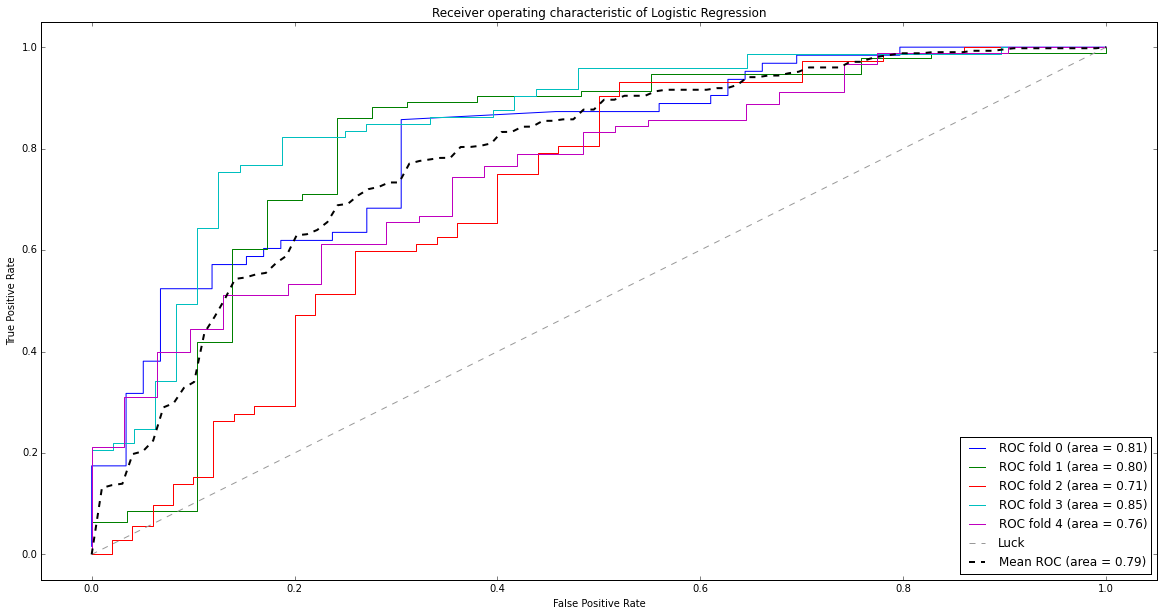
\includegraphics[width=\textwidth]{log_reg.png}
            \caption{Logistic Regression model Area under the ROC curve}
		\end{figure}
		\end{frame}

		\subsection{SVC evaluation}
		\begin{frame}
		\frametitle{SVC evaluation}
		\begin{figure}[h!]
        	\centering
            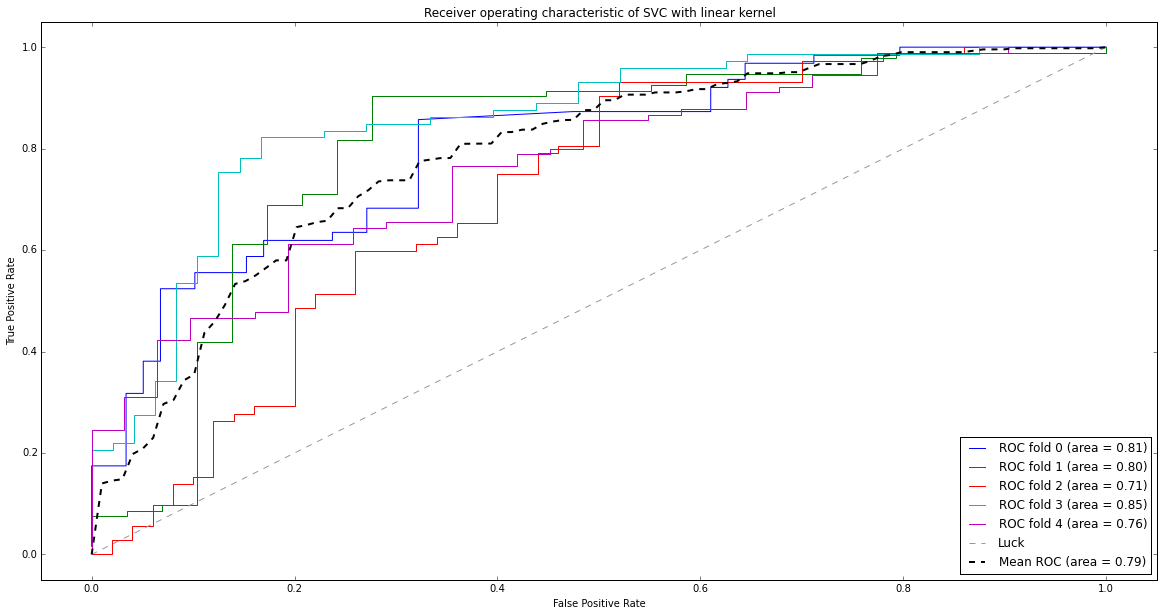
\includegraphics[width=\textwidth]{SVC.png}
            \caption{SVC model Area under the ROC curve}
		\end{figure}
		\end{frame}

		\subsection{LinearSVC evaluation}
		\begin{frame}
		\frametitle{LinearSVC evaluation}
		\begin{figure}[h!]
        	\centering
            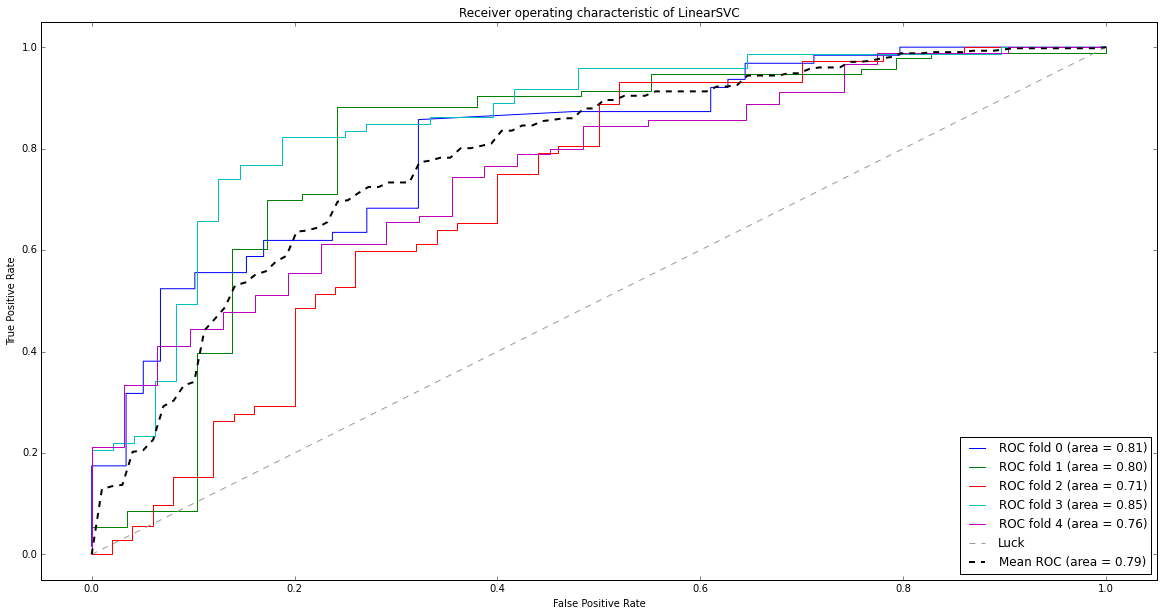
\includegraphics[width=\textwidth]{LinearSVC.png}
            \caption{LinearSVC model Area under the ROC curve}
		\end{figure}
		\end{frame}

	\section{Conclusion}
		\begin{frame}
		\frametitle{Conclusion}
			\begin{itemize}
				\item Difficult to handle the different currencies
				\item Difficult to normalize the incomes of the borrower (maybe transform it into categorical)
				\item Difficult to identify outliers into the borrowers (what criterion to use)
				\item Categorical feature are easier to use than numerical ones
				\item No real use of the temporal feature (no economic context)
				\item Improvement tracks :
				\begin{itemize}
					\item Use the lending club data
					\item Model the loan borrow as a Markov model (with a 6 months period for instance)
					\item In each step of the Markov process evaluate the risk
				\end{itemize}
			\end{itemize}
		\end{frame}


	\appendix
	\newcounter{finalframe}
	\setcounter{finalframe}{\value{framenumber}}
	% Backup frames
	\setcounter{framenumber}{\value{finalframe}}

\end{document}